% !TEX root = ../lectures_olympics.tex

\chapter{序言---写在前面}

什么是物理学?

相信大家经过小学自然科学和初中两年物理的学习,对物理已经有或多或少的了解。但是,在进入高中的物理学习之前,尤其是进入高中物理竞赛的学习之前,我们有必要仔细思考一下{\heiti 物理学}(physics)这个概念本身。这有益于我们确定我们的研究范围,合理地选取我们的研究方法。

首先,物理是一门{\heiti 自然科学}(nature science)。这就界定了物理学的{\heiti 研究对象}---自然现象。这一点把物理学同关心人与社会的人文学科区分开来,也把物理学同纯粹抽象的数学区分开来。再看物理学的{\heiti 研究方法}:一方面,物理学起源于古希腊的{\heiti 自然哲学}(nature philosophy)。它是一种依赖于经验的科学,大胆的猜想,定性的描述是古希腊很多关于物理的论述的特征。直至今天很多伟大的物理理论的诞生也离不开物理直觉与看似不直观的大但假设。

\begin{figure}[hbp]
\begin{minipage}[c]{0.6\textwidth}
\begin{center}
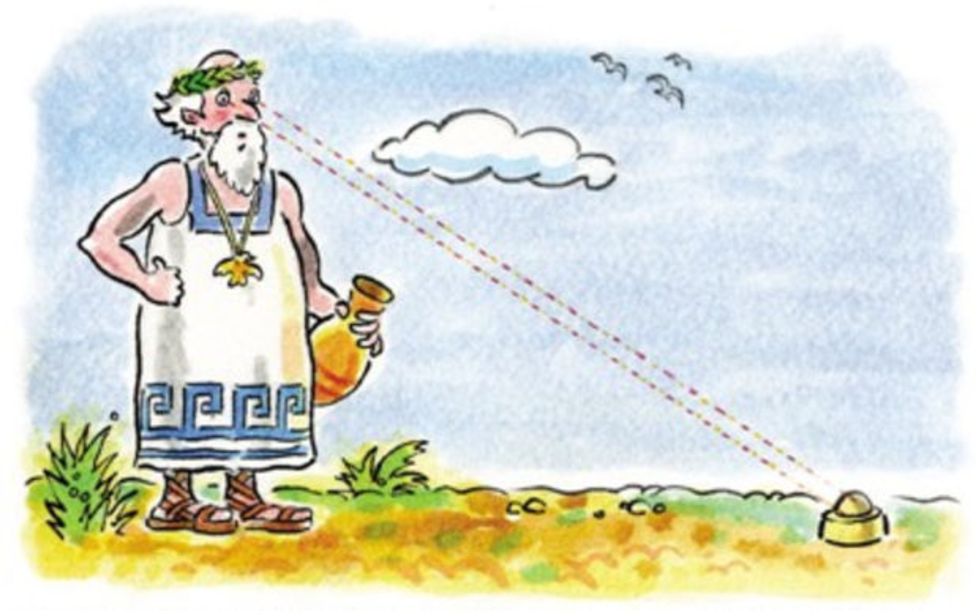
\includegraphics[height=2in]{images/pre_2.pdf}
\caption{毕达哥拉斯({\it Pythagoras})认为视觉来源于从眼睛里所发出的光的微粒仿佛触须一般落在了物体上,形成我们对物体的视觉感知。}
\end{center}
\end{minipage}
\hspace{1cm}
\begin{minipage}[c]{0.3\textwidth}
\begin{center}
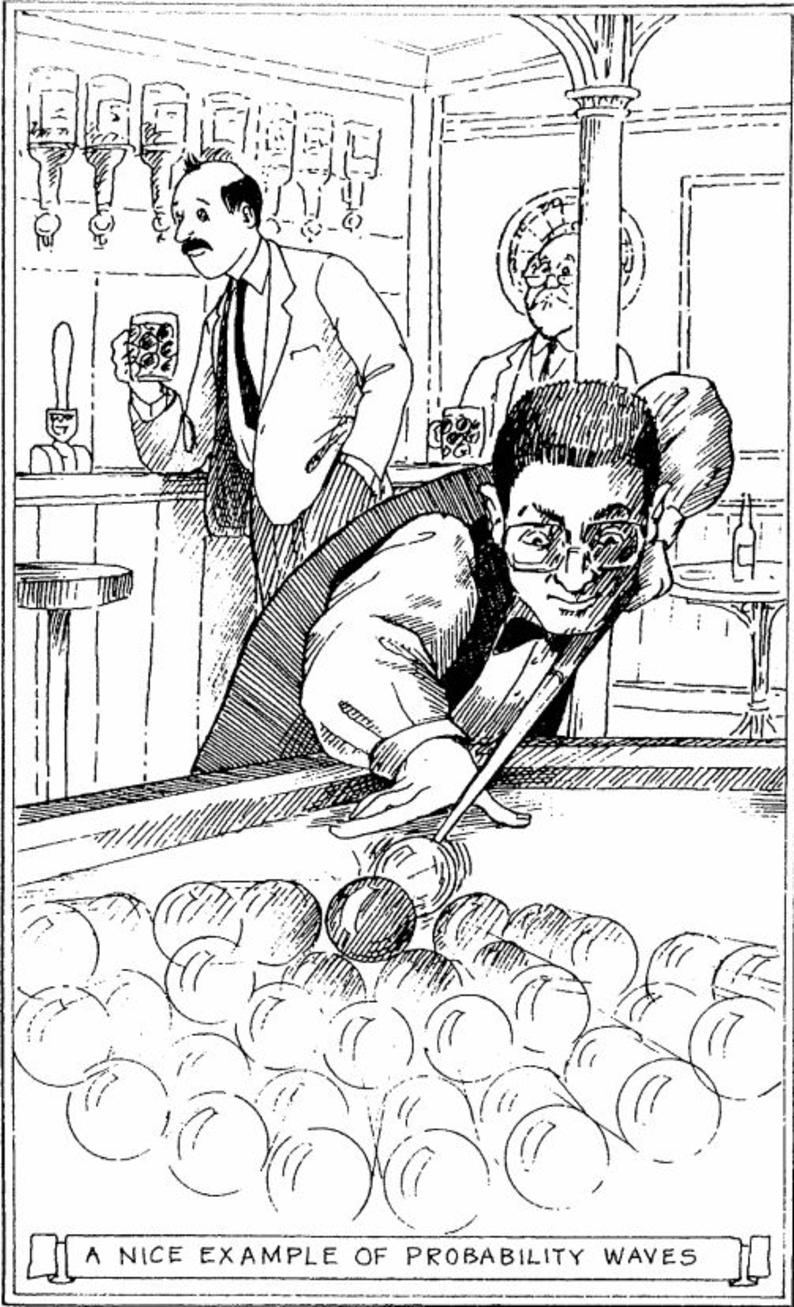
\includegraphics[height=2in]{images/pre_3.pdf}
\caption{海森堡({\it W. K. Heisenberg})等人认为微观粒子在运动过程中会``弥散''---仿佛一个量子台球会``分身术''一样。}
\end{center}
\end{minipage}
\end{figure}


另一方面,物理是{\heiti 实验科学}(experimental science)。它才从近代开始,就强烈地,而且越来越强烈地依赖于数学的定量逻辑推演和实验的验证。尤其是很多现代的物理学分支,往往不是物理猜想需要数学和实验去论证,而是在数学上的灵感和实验室里的发现带动了物理学的发展。例如1928年狄拉克({\it P. Dirac})将正常的粒子的运动规律方程在代数上进行了开平方运算,推导出了著名的狄拉克方程,一方面解释了电子的所谓自旋,一方面预言了电子的反物质---正电子的存在,电子与正电子相遇会湮灭并放出两个巨大能量的光子,这一发现翻开了粒子物理学的新篇章。再例如2002年和2015年两次获得诺贝尔奖的中微子\footnote{被认为是标准模型里基本粒子中最神秘的一类粒子,它质量极小又不为零,极难与物质参与相互作用所以非常难以探测。}探测实验,从更本上证明了所谓中微子振荡的存在,从而发现了中微子的非零质量,否定了物理学家们长期安心与信赖的标准模型。

\begin{wrapfigure}[12]{o}{6cm}
\begin{center}
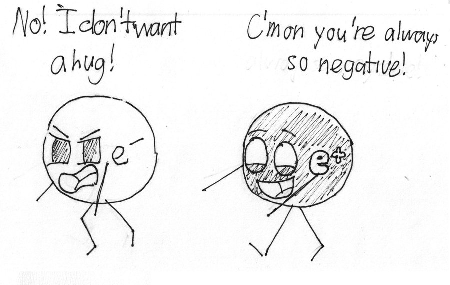
\includegraphics[width = 6cm]{images/pre_4.pdf}
\caption{电子与正电子是一对反粒子,相遇就会湮灭而消失}
\end{center}
\end{wrapfigure}

其次,我们要回答:物理包括哪些内容?我们即将学习的体系遵从了力学-热学-电磁学-光学-近代物理的顺序。知识编排从浅入深,并在合适的位置介绍微积分知识以备后用。但请同学们一定注意,这里给出的物理学分类既不是按照历史顺序,也没有照顾到以后普通物理,更深层次乃至物理前沿的分类方法。请同学们在学习本讲义的同时,兼顾了解你所学习的理论的前生今世,这样才有利于你进行进阶的学习。

最后,为什么学习物理?

学习物理,意味着用另一种思维方式去看待我们身边的世界。正如英国哲学家弗朗西斯$\cdot$培根({\it Francis Bacon}\footnote{没错,知识就是力量,法国就是培根!--Knowledge is Power, France is Bacon!})所说的:读史使人明智,读诗使人聪慧,演算使人精密,哲理使人深刻,道德使人有修养,逻辑修辞使人善辩。我们希望物理教育成为大家素质教育中的一环。希望大家通过物理的学习也能提高自己的涵养而不同流俗。另外,祖国对学习物理的我们给予了厚望。华夏子孙的发展与生存,不仅仅是经济的发展,它解决的是燃眉之急。若用长远的眼光来看,自然科学,尤其是物理学的发展与突破带来的是科学技术的创新,功在当代,利在千秋。最后,在学术的道路上中请谨慎选择自己的方向。物理既然可以成为人类发展的阶梯,也就能成为人类自取灭亡的灾厄。对一个学科的奉献往往需要牺牲精神。看看今日的科学与技术是如何发展起来的:布鲁诺为真理牺牲了生命,伽利略身陷囹吾,诺贝尔炸死了弟弟,居里夫人罹患白血病而亡......若为了科学事业牺牲了自己的青春,时间,家庭甚至爱情,那么我想这种精神即使不是可歌可泣的,多少也是宁人肃而起敬的。但若是为了科学事业迷失了自我,丧失了作为人的尊严,人性,道德,抑或是违背了学术活动的规范,急功近利,徇私舞弊,放弃了诚信与公平的原则。我想无论如何都是可悲的,是人类文化与教育的失败。

\begin{figure}[H]
\begin{center}
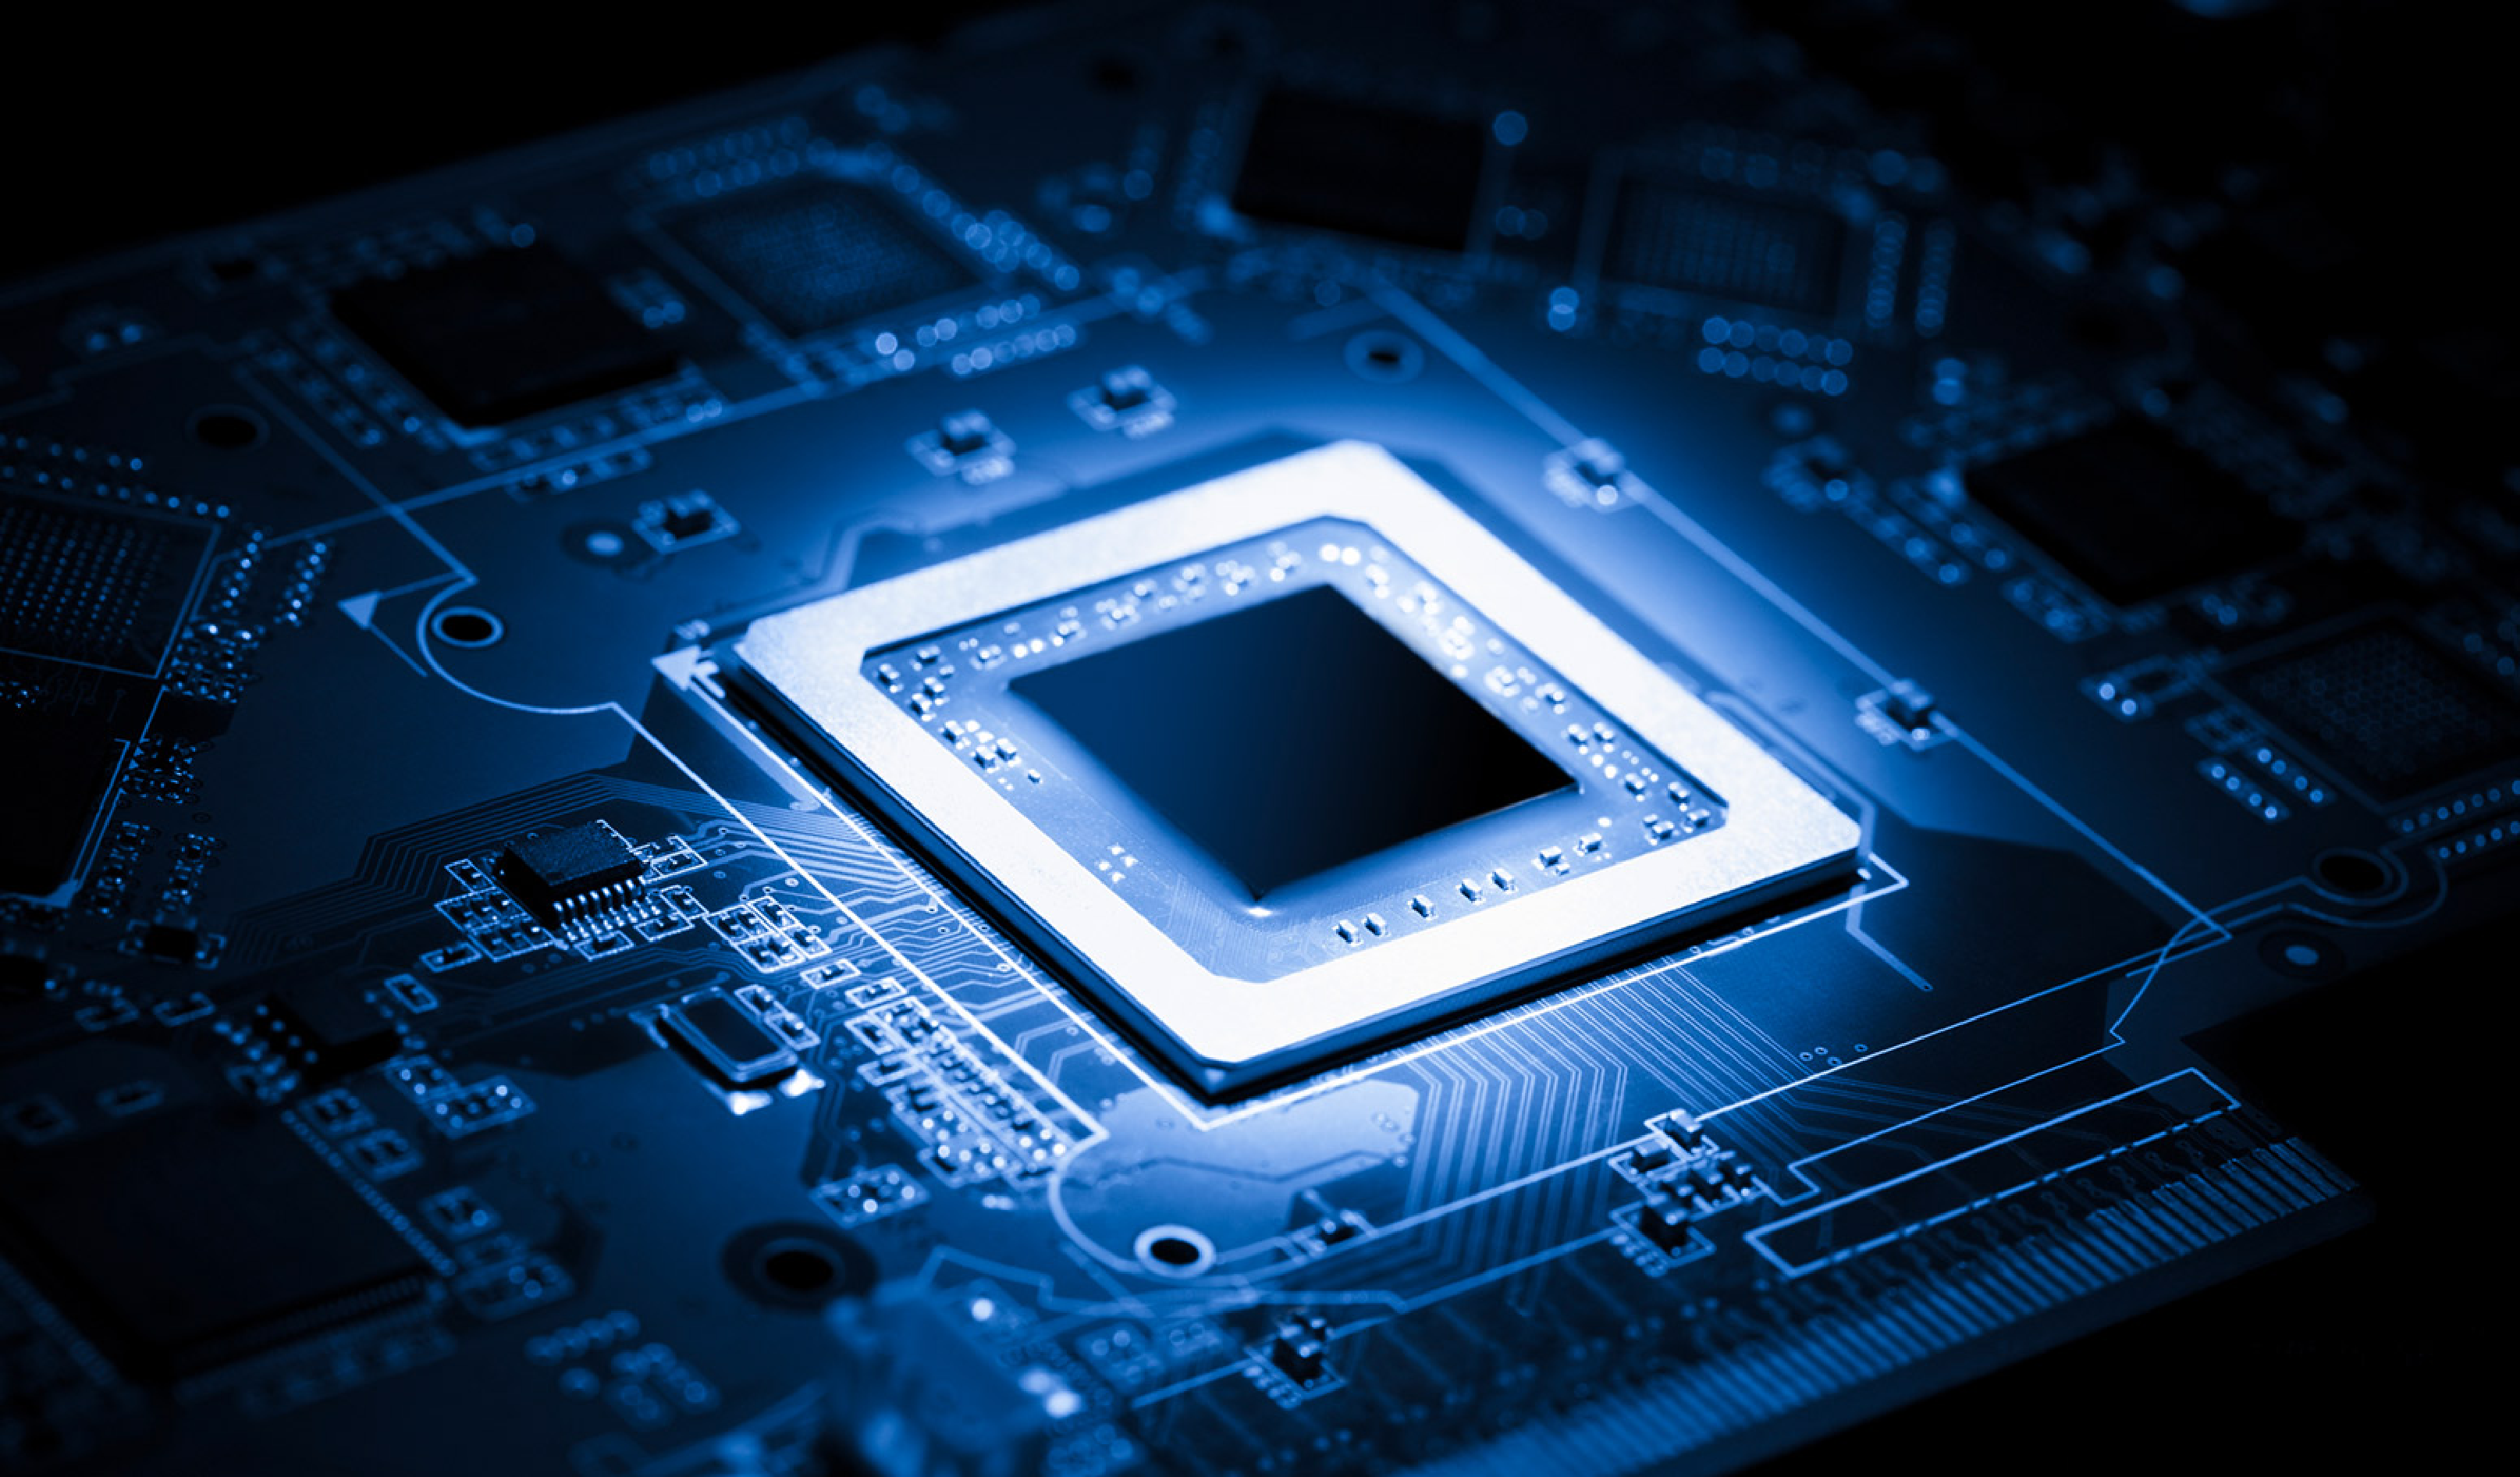
\includegraphics[height=1.5in]{images/pre_5.pdf}
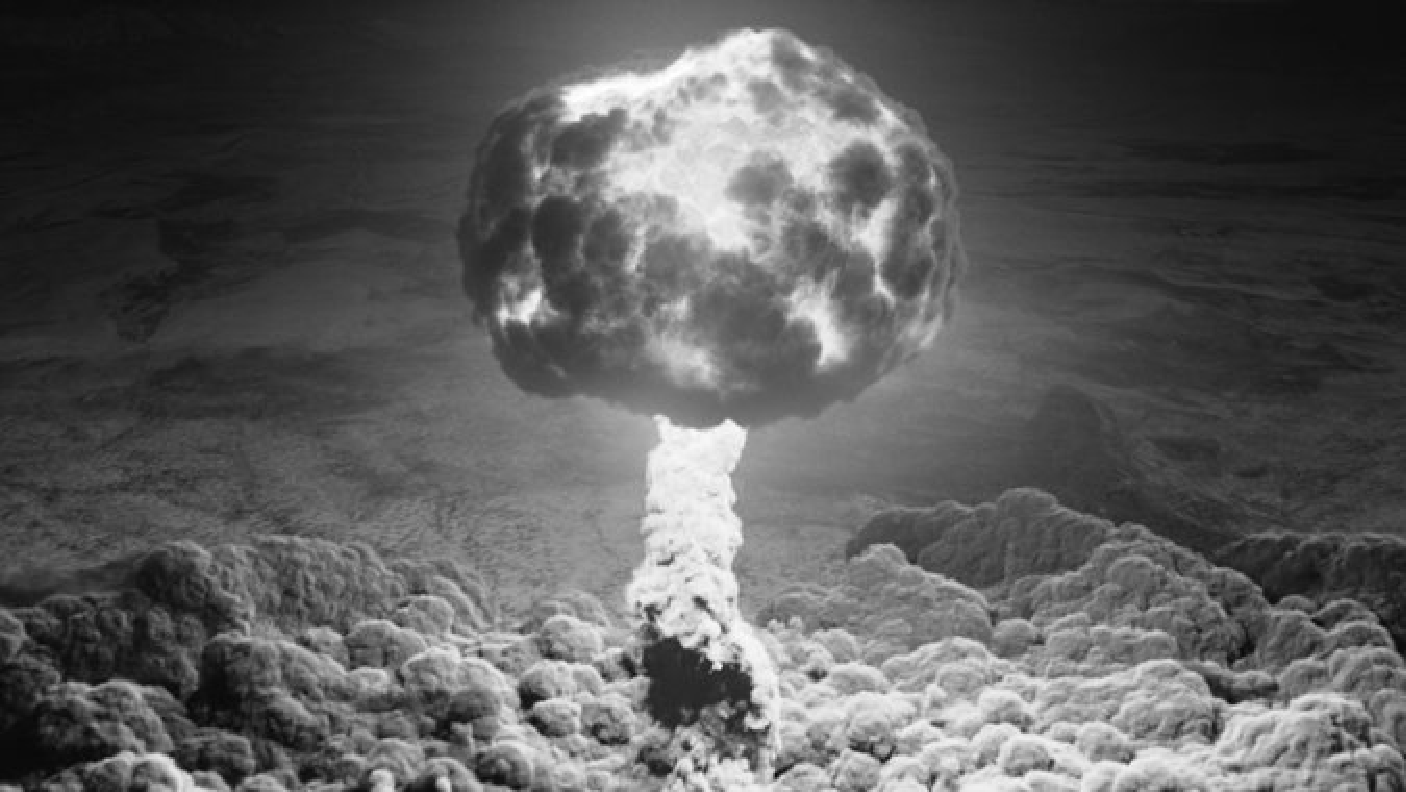
\includegraphics[height=1.5in]{images/pre_6.pdf}
\caption{量子力学给人类带来了半导体理论,半导体理论开启了信息时代的大门。图为集成电路,它是制作电子芯片的基础,我们身边的任何电子设备都离不开集成电路;量子力学也给人类带来了核能,核能带来了毁灭性的核武器。图为美国著名导演大卫$\cdot$林奇({\it David Lynch})所描绘的世界第一颗原子弹在新墨西哥州爆炸的场景。}
\end{center}
\end{figure}

所以在这里希望大家学习物理,不仅仅是因为物理有趣,对世界的未知吸引着你的好奇心,还是简单地享受物理学习过程中的成就感。请在学习过程中逐渐认清自己学习物理的目的,把个人对物理的喜爱升华为更崇高的追求。同时,我们也希望大家全面,均衡发展,培养广泛的思维方式和生活志趣,形成健全的人格。做一个对社会有益的公民。

最后,如果你问我喜欢物理的原因。我会告诉你:物理世界,异彩纷呈,正像那天上的星辰,玄之又玄,众妙之门。
\begin{figure}[H]
\begin{center}
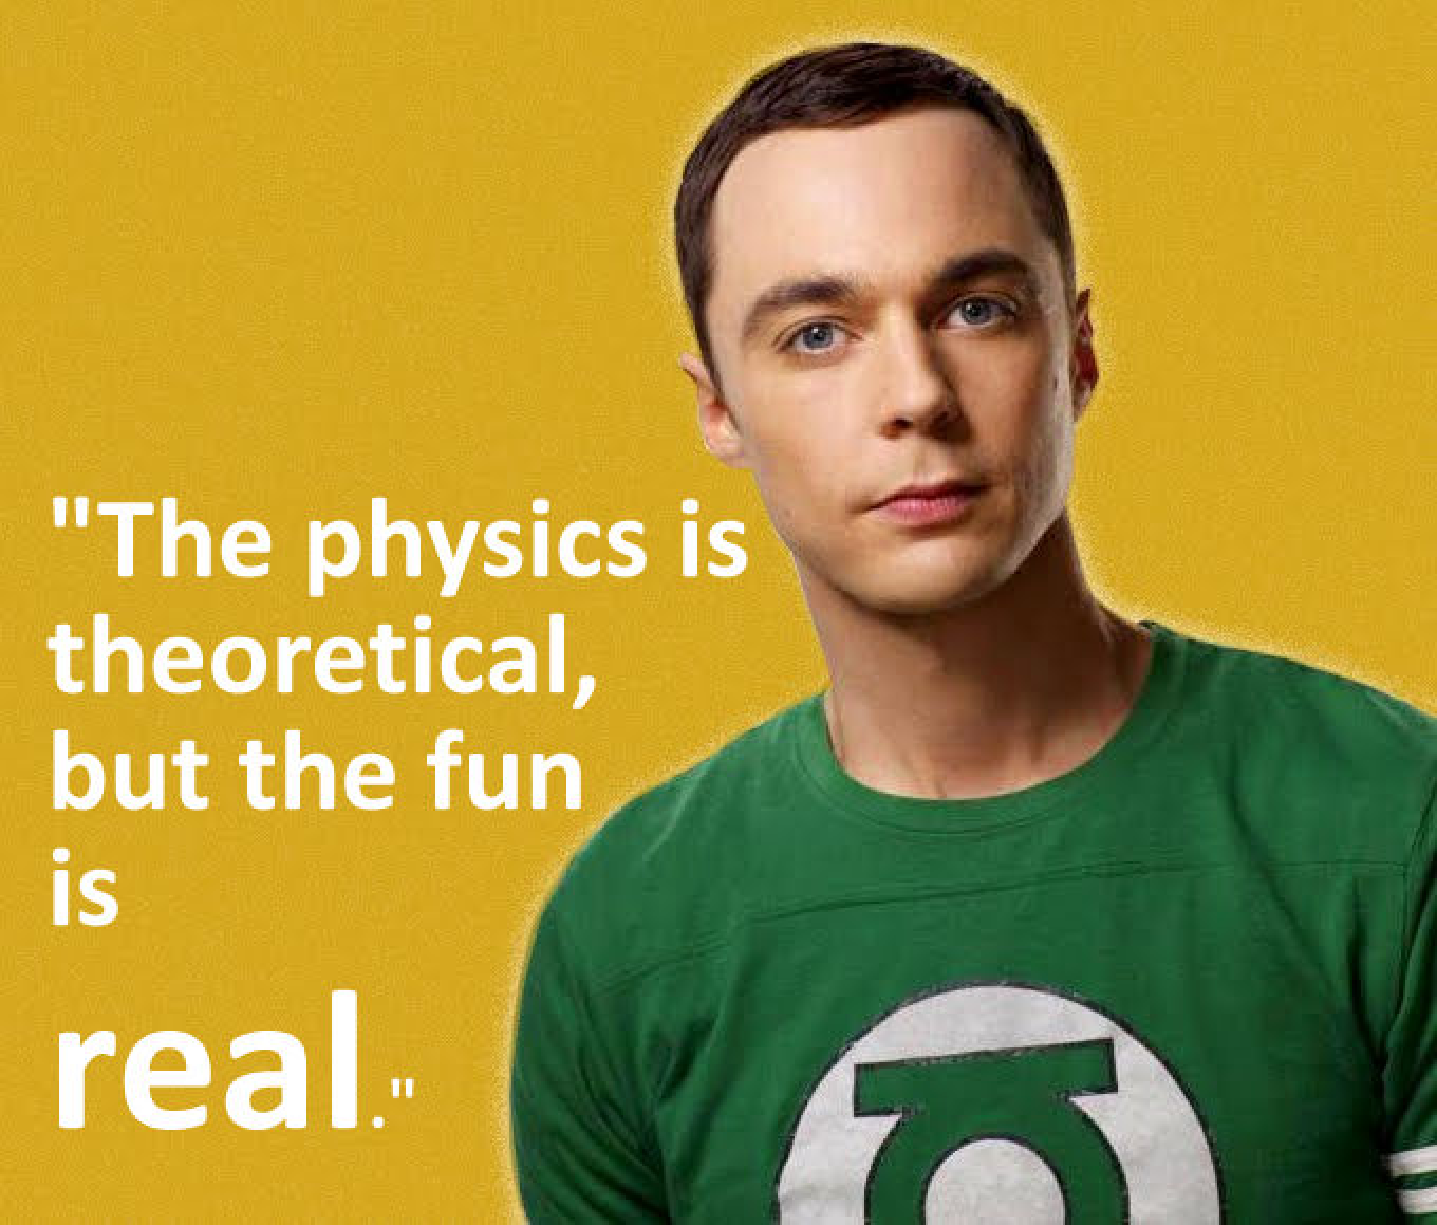
\includegraphics[height=3in]{images/pre_7.pdf}
\caption{美剧``{\kaishu 生活大爆炸}''里{\it Sheldon Cooper}发明的桌游``Research Lab''的口号}
\end{center}
\end{figure}
